\documentclass[aspectratio=43,english]{beamer} %If you want to create Polish presentation, replace 'english' with 'polish' and uncomment 3-th line, i.e., '\usepackage{polski}'
\usepackage[utf8]{inputenc}
\usepackage{polski} %Uncomment for Polish language
\usepackage{babel}
\usepackage{listings} %We want to put listings

\mode<beamer>{ 	%in 'beamer' mode
	\hypersetup{pdfpagemode=FullScreen}		%Enable Full screen mode
	\usetheme{JuanLesPins} 		%Show part title in right footer
	%\usetheme[dark]{AGH}                 		%Use dark background
	%\usetheme[dark,parttitle=leftfooter]{AGH}  	%Use dark background and show part title in left footer
}
\mode<handout>{	%in 'handout' mode
	\hypersetup{pdfpagemode=None}		
	\usepackage{pgfpages}
  	\pgfpagesuselayout{4 on 1}[a4paper,border shrink=5mm,landscape]	%show 4 slides on 1 page
  	\usetheme{boxes}
  	\addheadbox{structure}{\quad\insertpart\hfill\insertsection\hfill\insertsubsection\qquad} 	%content of header
 	\addfootbox{structure}{\quad\insertauthor\hfill\insertframenumber\hfill\insertsubtitle\qquad} 	%content of footer
}

\AtBeginPart{ %At begin part: display its name
	\frame{\partpage}
} 


%%%%%%%%%%% Configuration of the listings package %%%%%%%%%%%%%%%%%%%%%%%%%%
% Source: https://en.wikibooks.org/wiki/LaTeX/Source_Code_Listings#Using_the_listings_package
%%%%%%%%%%%%%%%%%%%%%%%%%%%%%%%%%%%%%%%%%%%%%%%%%%%%%%%%%%%%%%%%%%%%%%%%%%%%
\lstset{ %
  backgroundcolor=\color{white},   % choose the background color
  basicstyle=\footnotesize,        % the size of the fonts that are used for the code
  breakatwhitespace=false,         % sets if automatic breaks should only happen at whitespace
  breaklines=true,                 % sets automatic line breaking
  captionpos=b,                    % sets the caption-position to bottom
  commentstyle=\color{green},      % comment style
  deletekeywords={...},            % if you want to delete keywords from the given language
  escapeinside={\%*}{*)},          % if you want to add LaTeX within your code
  extendedchars=true,              % lets you use non-ASCII characters; for 8-bits encodings only, does not work with UTF-8
  frame=single,	                   % adds a frame around the code
  keepspaces=true,                 % keeps spaces in text, useful for keeping indentation of code (possibly needs columns=flexible)
  keywordstyle=\color{blue},       % keyword style
  morekeywords={*,...},            % if you want to add more keywords to the set
  numbers=left,                    % where to put the line-numbers; possible values are (none, left, right)
  numbersep=5pt,                   % how far the line-numbers are from the code
  numberstyle=\tiny\color{gray},   % the style that is used for the line-numbers
  rulecolor=\color{black},         % if not set, the frame-color may be changed on line-breaks within not-black text (e.g. comments (green here))
  showspaces=false,                % show spaces everywhere adding particular underscores; it overrides 'showstringspaces'
  showstringspaces=false,          % underline spaces within strings only
  showtabs=false,                  % show tabs within strings adding particular underscores
  stepnumber=2,                    % the step between two line-numbers. If it's 1, each line will be numbered
  stringstyle=\color{cyan},        % string literal style
  tabsize=2,	                   % sets default tabsize to 2 spaces
  title=\lstname,                  % show the filename of files included with \lstinputlisting; also try caption instead of title
                                   % needed if you want to use UTF-8 Polish chars
  literate={?}{{\k{a}}}1
           {?}{{\k{A}}}1
           {?}{{\k{e}}}1
           {?}{{\k{E}}}1
           {�}{{\'o}}1
           {�}{{\'O}}1
           {?}{{\'s}}1
           {?}{{\'S}}1
           {?}{{\l{}}}1
           {?}{{\L{}}}1
           {?}{{\.z}}1
           {?}{{\.Z}}1
           {?}{{\'z}}1
           {?}{{\'Z}}1
           {?}{{\'c}}1
           {?}{{\'C}}1
           {?}{{\'n}}1
           {?}{{\'N}}1
}
%%%%%%%%%%%%%%%%%


\title{Metody Obliczeniowe w Nauce i Technice}
\author{Marian Bubak, PhD}
\date{}
\institute[AGH]{
	Institute of Computer Science\\ul. Kawiory 21\\30-055 Krakow\\
	Poland\\
	\url{http://www.icsr.agh.edu.pl/~mownit/}
}



\subtitle{5. Aproksymacja}
\setcontributors{Paweł Urban, Jakub Ptak}


\begin{document}
  	\maketitle
  	\begin{frame}{Outline}
  			\tableofcontents
  	\end{frame}
	\section{Aproksymacja}
    %%%%%%%%%%%%%%%%
    \begin{frame}{Aproksymacja}
        Aproksymacja:
		\begin{itemize}
            \item przybliżanie, zastępowanie funkcji,
            \item jest ogólniejsza niż interpolacja
        \end{itemize}
    \end{frame}
	%%%%%%%%%%%%%%%%
    \begin{frame}{Funkcja aproksymowana i aproksymująca}
        $F(x)$ - to funkcja aproksymowana i może być:
        \begin{itemize}
          \item znana
          \item tablicą wartości eksperymentalnych (z błędami, a wtedy interpolacja nie ma sensu)
        \end{itemize}
        \hfill \break
        $f(x)$ - to funkcja aproksymująca = przybliżenie F(x)
	\end{frame}
	%%%%%%%%%%%%%%%%
	\section{Aproksymacja średniokwadratowa}
%%%%%%%%%%%%%%%%%%%
\begin{frame}{Aproksymacja średniokwadratowa}
  	\begin{figure}
	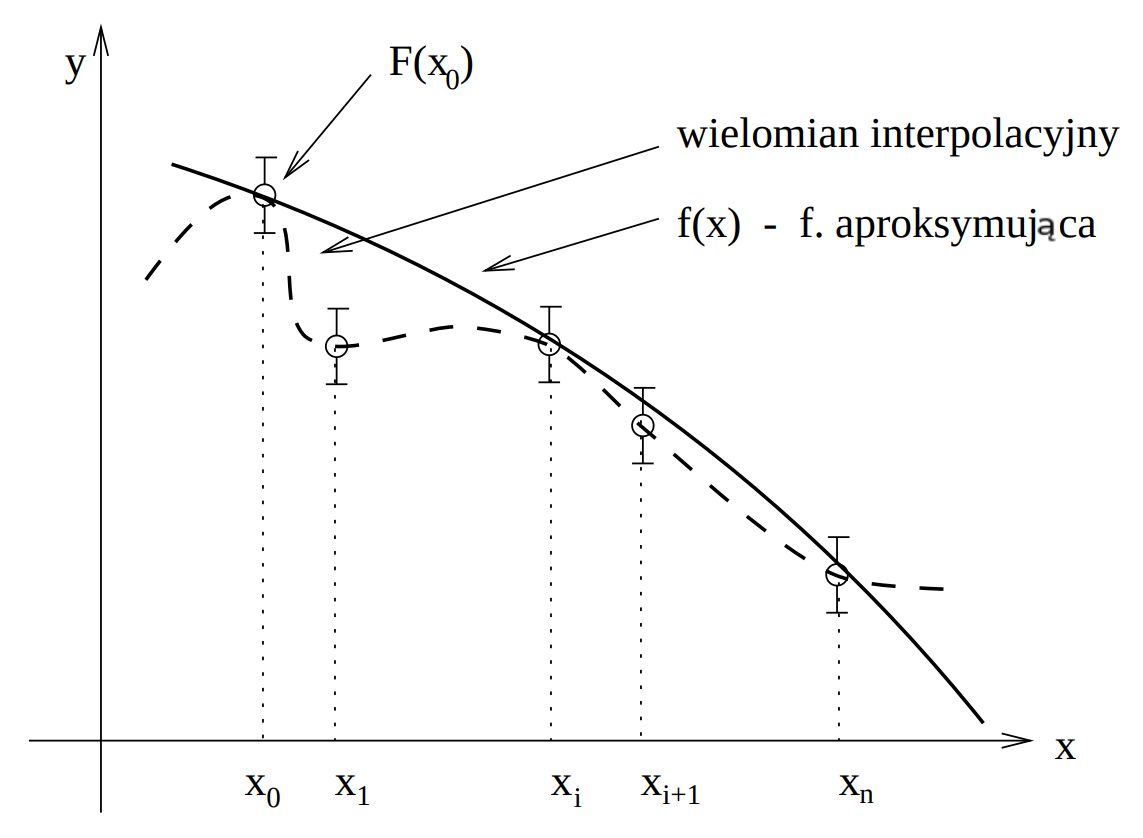
\includegraphics[height=0.8\textheight]{img/5/aproksymacja_sredniokwadratowa}
	\end{figure}
\end{frame}
%%%%%%%%%%%%%%%%%%%
\begin{frame}{Postawienie problemu}
	\textbf{Dane:}\newline
    - ${(x_i,y_i = F(x_i)),i=0,1,\ldots,n}$, czyli mamy (n+1) węzłów \newline
    - układ funkcji bazowych: $\varphi_j(x),j=0,1,\ldots,m$.\newline\par
    \textbf{Szukamy wielomianu uogólnionego:}
    $$f(x) = \sum_{j = 0}^{m} a_j \varphi_j(x)$$
    czyli $\{{a_j}\}_{j=0}^m$, dla których:
    $$min!\parallel F(x) - f(x) \parallel = min!\underbrace{ \sum_{i=0}^{n}w(x_i)\underbrace{\bigg[F(x_i)-\sum_{j=0}^{m}a_j\varphi_j(x_i)\bigg]^2}_\text{odchylenie}}_{H(a_0,a_1,\ldots,a_m)}$$
    \textbf{Pochodzenie nazwy:} postać normy $F(x)$ na $[a,b]$
\end{frame}
%%%%%%%%%%%%%%%%%%%
\begin{frame}{Przypadek ciągły}
	Dla przypadku ciągłego:
    $$min!\int_a^bw(x)[F(x)-f(x)]^2dx : \sum \rightarrow \int$$
    $\Rightarrow$ aproksymacja średniokwadratowa funkcji ciągłych\newline
    $w(x_i)$ - funkcja wagowa, $w(x_i)>0$ (jak dla iloczynu skalarnego) i zwykle: $w(x_i) \sim \frac{1}{[\text{błąd }F(x_i)]^2}$ \newline
\end{frame}
\begin{frame}{Współczynniki wielomianu uogólnionego}
    Współczynniki $\{a_j\}$ znajdujemy z warunku: $\frac{\partial H}{\partial a_k} = 0, k=0,1,\ldots,m$
    $\Rightarrow$ układ $(m+1)$ równań liniowych o $(m+1)$ niewiadomych
    $$\frac{\partial H}{\partial a_k} = -2 \cdot \sum_{i=0}^{n}w(x_i)\bigg[F(x_i)-\sum_{j=0}^{m}a_j\varphi_j(x_i)\bigg]\varphi_k(x_i)=0;k=0,1,\ldots,m$$
    Jest to \textbf{układ normalny.}
\end{frame}
%%%%%%%%%%%%%%%%%%%
\begin{frame}{Aproksymacja wielomianowa}
	funkcje bazowe $\rightarrow$ ciąg jednomianów $\varphi_j(x) = x^j,j=0,1,\ldots,m$\newline
    funkcje aproksymująca: $f(x) = \sum_{j=0}^{m}a_j\varphi_j(x)=\sum_{j=0}^{m}a_jx^j$ \newline
    $F(x)$ - na zbiorze dyskretnym $\{x_i\},i=0,1,\ldots,n$
    $$min!\sum_{i=0}^{n}w(x_i)[F(x_i)-f(x_i)]^2 \rightarrow$$
    układ normalny:
    $$\sum_{i=0}^{n}w(x_i)\bigg[F(x_i)-\sum_{j=0}^{m}a_jx_i^j\bigg]x_i^{k\leftarrow\frac{\partial f}{\partial a_k}}=0,k=0,1,\ldots,m$$
    $$\sum_{i=0}^{n}w(x_i)x_i^k\sum_{j=0}^{m}a_jx_i^j=\sum_{i=0}^{n}w(x_i)F(x_i)x_i^k,k=0,1,\ldots,m$$
    $$\sum_{j=0}^{m}\underbrace{\bigg(\sum_{i=0}^{n}w(x_i)x_i^{j+k}\bigg)}_{g_{k,j}}a_j = \underbrace{\sum_{i=0}^{n}w(x_i)F(x_i)x_i^k}_{b_k}$$
\end{frame}
%%%%%%%%%%%%%%%%%%%
\begin{frame}
	W postaci macierzowej:
    \begin{center}
    	 $\left(\begin{array}{ccccc}
    \sum w_i & \sum w_ix_i & \sum w_ix_i^2 & \ldots & \sum w_i x_i^m \\
    \sum w_ix_i & \sum w_ix_i^2 & \sum w_ix_i^3 & \ldots & \sum w_i x_i^{m+1} \\
    . & . & . & . & . \\
    \sum w_ix_i^m & \sum w_ix_i^{m+1} & \sum w_ix_i^{m+2} & \ldots & \sum w_i x_i^{2m}
    \end{array}\right)
    \left(\begin{array}{c}
    	a_0 \\ a_1 \\ \vdots \\ a_m
    \end{array}\right) =\newline=
    \left(\begin{array}{c}
    	\sum w_iF_i\\
        \sum w_i F_i x_i \\
        \vdots \\
        \sum w_i F_i X_i^m
    \end{array}\right)$
    \end{center}
    \begin{center}
    	\underline{$G \cdot A = B$}
    \end{center}
   	
\end{frame}
%%%%%%%%%%%%%%%%%%%
\begin{frame}
	\textbf{Jeżeli:}
    \begin{enumerate}
    \item $x_0,x_1,\ldots,x_n$ - są różne
    \item $m \leqslant n$
    \end{enumerate}
    to $det G \not= 0 \rightarrow$ układ ma jedno rozwiązanie. 
    \begin{flushright}
    	\textit{Zadanie: } \quad Pokazać, że dla $m = n$ - wiel. aproksymacyjny = interpolacyjny $(H=0)$
     \end{flushright}
\end{frame}
%%%%%%%%%%%%%%%%%%%
\begin{frame}{W praktyce}
	\begin{itemize}
	\item $m \ll n$ (korzystamy z dużej ilości informacji)
    \item $m$ - wysoki - by dobrze przybliżyć funkcję
    \item $m$ - niski - by wygładzić błędy
    \item zwykle $m \leqslant 6$
	\end{itemize}
\end{frame}
%%%%%%%%%%%%%%%%%%%
\begin{frame}{Ortogonalność funkcji}
	\begin{block}{Definicja ortogonalności funkcji}
	Funkcje $f(x)$ i $g(x)$ nazywamy ortogonalnymi na dyskretnym zbiorze punktów $\{x_i,i=0,1,..,n\}$ jeżeli:
    $$\sum_{i=0}^{n}f(x_i)\cdot g(x_i) = 0, \sum_{i=0}^{n}[f(x_i)]^2 > 0,\sum_{i=0}^{n}[g(x_i)]^2 > 0$$
	\end{block}
\end{frame}
%%%%%%%%%%%%%%%%%%%
\begin{frame}{Ortogonalność ciągów}
	\begin{block}{Definicja ortogonalności ciągów}
	Ciągi funkcyjne $\{\varphi_k(x)\}$ nazywamy ortogonalnymi na dyskretnym zbiorze punktów $\{x_i\}$ jeśli:
    $$\sum_{i=0}^{n}\varphi_j(x_i)\varphi_k(x_i) = \left\{\begin{array}{cl}
    	0 & j \not= k \\
        >0 & j = k \quad \rightarrow (*)
    \end{array}\right.$$
    $(*)$ - nie wszystkie $x_i$ to miejsca zerowe.
	\end{block}
\end{frame}
%%%%%%%%%%%%%%%%%%%
\begin{frame}{Aproksymacja średniokwadratowa wielomianami ortogonalnymi}
	Dla wielomianów ortogonalnych układ normalny:
    $$\sum_{i=0}^{n}w(x_i)\Bigg[F(x_I)-\underbrace{\sum_{j=0}^{m}a_j\varphi_j(x_i)}\Bigg]\varphi_k(x_i)=0,k=0,1,..,m$$
    \begin{center}
    	$$\sum_{i=0}^{n}w(x_i)\varphi_k(x_i)\sum_{j=0}^{m}a_j\varphi_j(x_i)=$$\newline$$=\sum_{j=0}^{m}a_j\sum_{i=0}^{m}w(x_i)\varphi_k(x_i)\varphi_j(x_i) = a_k\sum_{i=0}^{n}W_i\varphi_k^2(x_i)$$
    \end{center}
    
\end{frame}
%%%%%%%%%%%%%%%%%%%
\begin{frame}
	$\rightarrow$ macierz staje się diagonalna $\rightarrow$ znika:
    \begin{itemize}
    \item złe uwarunkowanie
    \item konieczność ponowanego rozwiązywania układu normalnego przy zmianie stopnia wielomianu aproksymującego
    \end{itemize}
	Najczęściej stosowane wielomiany ortogonalne:
    \begin{itemize}
    \item Czebyszewa $T_j(x)$
    \item Legendre'a $P_n(x)$ ($\rightarrow$ zwłaszcza dla $w(x_i) = 1$)
    \end{itemize}
\end{frame}
%%%%%%%%%%%%%%%%%%%
\begin{frame}{Aproksymacja średniokwadratowa funkcjami sklejanymi}
	\begin{flushright}
		\textit{Zadanie:} \quad Pokazać, że: $f(x) = s(x)$
	\end{flushright}
\end{frame}
%%%%%%%%%%%%%%%%%%%
\begin{frame}{Wielomiany Legendre'a}
	Określone wzorem $P_n(x) = \frac{1}{n!2^n}\frac{d^n}{dx^n}[(x^{-1})^n],x \in [-1,1], n = 0,1,\ldots$
    Spełniają wzór rekurencyjny:
    $$(2n+1) \cdot x \cdot P_n(x)=(n+1)P_{n+1}(x)+n \cdot P_{n-1}(x)$$
    \begin{flushleft}
    	$$\left.\begin{array}{l}
    P_0 = 1 \\
    P_1(x) = x \\
    P_2(x) = \frac{1}{2}(3x^2-1)\\
    P_3(x) = \frac{1}{2}(5x^3-3x) \\
    P_4(x) = \frac{1}{8}(35x^4-30x^2+3)\\
    \vdots \\
    P_n(1) = 1; |P_n(x)| \leqslant 1, x \in [-1,1]
    \end{array}\right.$$
    \end{flushleft}
\end{frame}
%%%%%%%%%%%%%%%%%%%
\begin{frame}
	\begin{figure}
		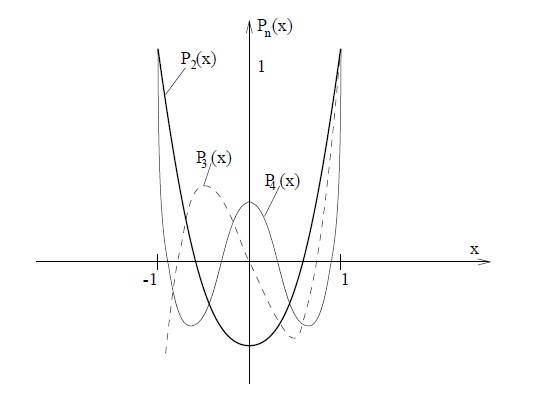
\includegraphics[height=0.82\textheight]{img/5/img2.jpg}
	\end{figure}
\end{frame}
%%%%%%%%%%%%%%%%%%%
\begin{frame}
	\begin{flushright}
    	\textit{Zadanie:} \quad Pokazać, że $P_n(-x) = (-1)^n \cdot P_n(x)$ 
    \end{flushright}
	spełniają równania różniczkowe:
        $$\frac{d}{dx}\bigg[(1-x^2)\frac{dP_n(x)}{dx}\bigg]+n(n+1)P_n(x) = 0$$
        (wynik rozdzielania zmiennych w r. Laplace'a we współrzędnych sferycznych) \newline \par
        \textbf{Ortogonalność: }
        $$\int_{-1}^{1}P_n(x)P_m(x)dx = \left\{\begin{array}{cc}
        0, & m \not= n \\
        \frac{2}{2n+1}, & m = n 
        \end{array}\right.$$
        \begin{flushright}
        	\textit{Zadanie: } \quad Sprawdzić ortogonalność w przypadku dyskretnym.
        \end{flushright}
\end{frame}
%%%%%%%%%%%%%%%%%%%

    \section{Aproksymacja jednostajna}
%%%%%%%%%%%%%%%%%%%
\begin{frame}
	Dla $F(x)$ określonej na $[a,b]$ szukamy $f(x)$:
    $$min! (\mathbf{F(x)-f(x)}) = min!\underbrace{sup_{x \in [a,b]}|F(x)-f(x)|}_{\text{norma Czebyszewa}}$$
\end{frame}
%%%%%%%%%%%%%%%%%%%
\begin{frame}
	\begin{block}{Twierdzenie Weierstrassa}
	Jeżeli $F(x) \in C^0[a,b]$, to dla każdego $\varepsilon>0$ można dobrać $n(\varepsilon)$ takie, że istnieje $W_n(x): |F(x)-W_n(x)|<\varepsilon$ \newline
    \newline Wniosek: $F(x)$ można aproksymować jednostajnie wielomianami.
	\end{block}
    Szukamy $a_i$:\newline
    $W_n(x) = \sum_{i=0}^{n}a_ix^i$ aby $min!E_n$, \newline
    $E_n = max_{x \in [a,b]} |F(x) - W_n(x)|$
\end{frame}
%%%%%%%%%%%%%%%%%%%
\begin{frame}
	\begin{block}{Twierdzenie Borela}
		Jeśli $F(x)\in C^0[a,b], n$ - naturalna, to istnieje $W_n(x)$ będący najlepszym przybliżeniem $F(x)$.
	\end{block}
    \begin{block}{Twierdzenie Czebyszewa}
    	Wielomian $W_n(x)$ będący najlepszym przybliżeniem $F(x)$ jest tylko jeden.
    \end{block}
\end{frame}
%%%%%%%%%%%%%%%%%%%
\begin{frame}{Metoda szeregów potęgowych - szereg Taylora}
	$$W_n(x) = \sum_{k=0}^{n}\frac{F^{(k)}(x_0)}{k!}(x-x_0)^k$$
    oszacowanie błędu aproksymacji $\rightarrow$ reszta Lagrange'a:
    $$F_n(x)-W_n(x) = \frac{F^{n+1}(\eta)}{(n-1)!}(x-x_0)^{n+1},\eta \in [a,b]$$
\end{frame}
%%%%%%%%%%%%%%%%%%%
\begin{frame}{Przybliżenia Padé}
	\textbf{ang.} Padé approximation, rational function approximation \newline
    \newline
    Funkcja wymierna $r(x)$ stopnia $N$ ma postać:
    $$r(x) = \frac{p(x)}{q(x)} = \frac{p_0+p_1(x)+\ldots+p_nx^n}{q_0+q_1(x)+\ldots+q_mx^m}$$
    \begin{itemize}
    \item nieredukowalna (p, q - są względnie pierwsze - nie mają wspólnych podzielników)
    \item określona w $x=0\Rightarrow q_0 \not = 0, \Rightarrow q_0=1$ (zwykle)
    \item do określenia $N+1 = n+m+1$ współczynników
    \end{itemize}
\end{frame}
%%%%%%%%%%%%%%%%%%%
\begin{frame}{Technika aproksymacji Padé}
	Jest to sposób określenia $\{p_i,q_j\}, i = 0,..,n,j = 0,..,m$ przy zadanych $n,m$ - możliwie najwięcej pochodnych $F(x)$ i $r(x)$ w $x=0\rightarrow$ równych!
    $$F(x) - r(x) = F(x) - \frac{p(x)}{q(x)}=\frac{F(x) \cdot q(x) - p(x)}{q(x)}$$
    Niech $F(x) = \sum_{i=0}^{\infty}a_i \cdot x^i \rightarrow$ szereg Maclaurina
    $$F(x) - r(x) = \frac{\sum_{i=0}^{\infty}a_ix^i \cdot \sum_{i=0}^{m}q_ix^i - \sum_{i=0}^{n}p_ix^i}{q(x)}$$
    Należy dobrać $p_0,p_1,..,p_n$ i $q_1,..,q_m$ tak, aby:
    $$F^{(k)}(0)-r^{(k)}(0) = 0, k=0,1,..,N$$
    
\end{frame}
%%%%%%%%%%%%%%%%%%%
\begin{frame}
	\begin{flushright}
		\textit{Zadanie: } \quad Pokazać, że jest to równoważne z: \newline\textit{$(F-r)$ ma w $x=0$ pierwiastek $N+1$ krotny.}
	\end{flushright}
    To znaczy, że licznik:
    $$(a_0+a_1x+..)(1+q_1x+..+q_mx^m)-(p_0+p_1x+..+p_nx^n)$$
    nie powinien mieć wyrazów stopnia $\leqslant N$. Dla uproszczenia zapisu:
    \begin{center}
    	$p_{n+1} = p_{n+2}=..=p_N=0$ i $q_{m+1} = q_{m+2} = .. =q_N = 0$
    \end{center}
    Wtedy współczynniki: $\sum_{i=0}^{k}a_iq_{k-1}-p_k$, a znalezienie $p(x)$ i $q(x)$ polega na rozwiązaniu układu równań liniowych:
    $$\sum_{i=0}^{k}a_iq_{k-1}-p_k = 0;k=0,1,...,N$$
\end{frame}
%%%%%%%%%%%%%%%%%%%
\begin{frame}{Typowy przykład}
	$$(*) \rightarrow F(x) = \big[7+(1+x)^{\frac{4}{3}}\big]^{\frac{1}{3}} \approx 2+\frac{1}{9}x+\frac{1}{81}x^2-\frac{49}{8748}x^3+\frac{175}{78732}x^4+\ldots $$
    \begin{block}{Uwagi}
    	\begin{itemize}
    	\item twierdzenie o zbieżności $r(x) \leftarrow$ dod. zał. o $F(x)$
        \item w praktyce: $N = n+m$ - ustalone: $\left\{\begin{array}{ccl}
        	n & = & m \\
            n & = & m+1
        \end{array}\right.$
    	\end{itemize}
    \end{block}
\end{frame}
%%%%%%%%%%%%%%%%%%%

    \section{Wielomiany Czebyszewa (Chebyshev Polynomials)}
%%%%%%%%%%%%%%%%%%%
\begin{frame}{Reprezentacja trygonometryczna}
	$$\cos(n\varphi)+\cos[(n-2)\varphi] = 2\cos[(n-1)\varphi] \cdot \cos \varphi$$
    $$\cos(n\varphi) = 2\cos[(n-1)\varphi] \cdot \cos \varphi - \cos[(n-2)\varphi]$$
    dla $x \in [-1,1]\Rightarrow \varphi=\arccos x$
    $$T_n(x) = \cos[n \cdot \arccos x]$$
\end{frame}
%%%%%%%%%%%%%%%%%%%
\begin{frame}{Relacja rekurencyjna}
	\begin{tabular}{l}
		$T_0(x) = 1$ \\
        $T_1(x) = x$ \\
        $T_2(x) = 2x^2-1$ \\
        $T_3(x) = 4x^3-3$ \\
        $T_4(x) = 8x^4-8x^2+1$ \\
        $T_5(x) = 16x^5-20x^3+5x\ldots$ \\
        $\vdots$ \\
        $T_n(x) = 2xT_{n-1}(x) - T_{n-2}(x), dla n\geqslant2$
	\end{tabular}
    
    \begin{block}{Czynnik wiodący}
    	Czynnik wiodący w $T_n(x)$ jest to czynnik przy najwyższej potędze $x$, czyli $2^{n-1} (dla n\geqslant1)$
    \end{block}
\end{frame}
%%%%%%%%%%%%%%%%%%%
\begin{frame}{Symetria}
	$$T_k(-x)=(-1)^k \cdot T_k(x)$$
    \begin{figure}
		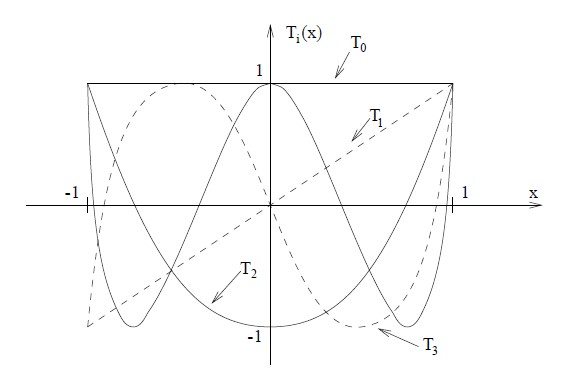
\includegraphics[height=0.75\textheight]{img/5/symetria.jpg}
	\end{figure}
\end{frame}
%%%%%%%%%%%%%%%%%%%
\begin{frame}{Miejsca zerowe $T_n(x)$ - węzły Czebyszewa}
	$T_n(x)$ ma w $[-1,1]$ $n$ miejsc zerowych:\newline
    $x_k = \cos (\frac{2k+1}{n} \cdot \frac{\pi}{2}), k=0,1,..,n-1$
    $$T_n(x) = \cos(n \underbrace{\arccos x}_\alpha)$$
    $$\cos(n \cdot \alpha) = 0 \text{ dla } n \cdot \alpha = (2k+1) \cdot \frac{\pi}{2},k=0,1,..,n-1$$
\end{frame}
%%%%%%%%%%%%%%%%%%%
\begin{frame}{Ortogonalność}
	\begin{block}{Przypadek ciągły}
		$$\int_{-1}^{1}\frac{T_i(x) \cdot T_j(x)}{\sqrt{1-x^2}}dx = \left\{\begin{array}{lc}
			0 & i \not= j \\
            \frac{\pi}{2} & i = j \not= 0 \\
            \pi & i = j = 0 \rightarrow \text{repr. tryg.}
		\end{array}\right.$$
	\end{block}
    
    \begin{block}{Przypadek dyskretny $x_k - miejsca zerowe T_{m+1}(x)$}
    $$\sum_{k=0}^{m}T_i(x_k)T_j(x_k) = \left\{\begin{array}{rc}
    	0 & i \not= j \\
        \frac{m+1}{2} & i=j \not= 0 \\
        m+1 & i=j=0
    \end{array}\right.$$
    \end{block}
\end{frame}
%%%%%%%%%%%%%%%%%%%
\begin{frame}{Własność minimaksu wielomianów Czebyszewa}
	\begin{block}{Twierdzenie o normie $T_n(x)$}
		Ze wszystkich wielomianów stopnia $n\geqslant1$ z czynnikiem wiodącym równym 1 najmniejszą normę maksymalną w $[-1,1]$
        $$\lVert W_n \rVert _{\infty} = max_{x \in [a,b]}|W_n|$$
        ma wielomian $2^{1-n} \cdot T_n(x)$. Wynosi ona $2^{1-n}$
	\end{block}
\end{frame}
%%%%%%%%%%%%%%%%%%%
\begin{frame}
	\textbf{Dowód (nie wprost) }\newline
	\begin{tabular}{|l}
		Załóżmy, że $\exists p_n(x)$ o współczynniku wiodącym = 1 taki, że:
      \\$\forall_{x \in [-1,1]}|p_n(x)| < 2^{1-n}$ wszystkie $T_n(1) = 1$, $x = 1$\\ $\Rightarrow x_0'$ (punkt ekstremalny) \\
	\end{tabular}	
    \begin{figure}
		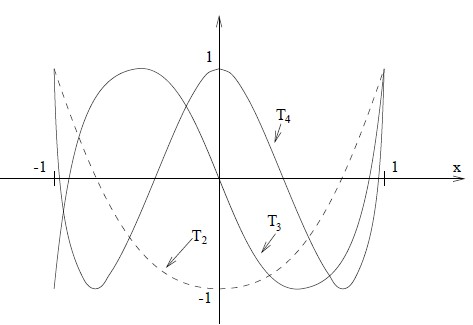
\includegraphics[height=0.7\textheight]{img/5/dowod.jpg}
	\end{figure}
\end{frame}
%%%%%%%%%%%%%%%%%%%
\begin{frame}
	\begin{tabular}{|l}
		Odcięta punktu ekstremalnego $T_n(x)$, $x_k'=\cos\frac{k\pi}{n}$, $k=0,1,..,n$\\
        Dla $\forall x_k'$ powinno zachodzić: \\
        $p_n(x_0') < 2^{1-n} \cdot T_n(x_0')$, \\
        $p_n(x_1') > 2^{1-n} \cdot T_n(x_1')$, \\
        $p_n(x_2') < 2^{1-n} \cdot T_n(x_2')$, \\
        \ldots , aż do $x_n'$ \\
        $\Rightarrow$ czyli wielomian $[p_n(x) - 2^{1-n} \cdot T_n(x)]$ \\
        powinien zmieniać znak w każdym z przedziałów: \\
        $(x_{k+1}',x_k')$, $k = \underbrace{n-1, n-2,..,1,0}_{\text{n przedziałów $\rightarrow$ n zer}} $\\ 
         $\Rightarrow $ czyli powinien być wielomianem stopnia $n$ w $[-1,1]$, \\ 
         ale $p_n(x)$ i $2^{1-n} \cdot T_n(x)$ mają ten sam współczynnik wiodący, \\
         Zatem ich różnica jest stopnia $n-1$ i mamy sprzeczność!!!
	\end{tabular}
\end{frame}
%%%%%%%%%%%%%%%%%%%
\begin{frame}{Aproksymacja wielomianami Czebyszewa}
	$\rightarrow$ jednostajna: $min!sup_{x \in [a,b]}|F(x)-f(x)|$ \newline
    baza $T_i(x)$ wygodna, bo $T_i(x)$ - równomierne w $[-1,1]$ \newline
    $F(x)$ \textbf{zastępujemy sumą częściową:}
    $$F(x) \approx \sum_{j=0}^{N}c_jT_j(x)$$
    z $c_j$ wyznaczonymi z warunku ortogonalności w przypadku ciągłym
    $$F(x) = \sum_{j=0}^{\infty}c_jT_j(x)    \bigg\arrowvert \cdot\frac{T_i(x)}{\sqrt{1-x^2}}  \bigg\arrowvert \int_{-1}^{1}dx$$
    \begin{tabular}{ll}
    $c_0 = \frac{1}{\pi}\int_{-1}^{1}\frac{F(x)T_i(x)dx}{\sqrt{1-x^2}}$ &
    $c_i = \frac{2}{\pi}\int_{-1}^{1}\frac{F(x)T_i(x)dx}{\sqrt{1-x^2}}, i=1,..,N$
    \end{tabular}
    
    Często - zamiast $\uparrow \rightarrow$ interpolacja $T_{n+1}(x)$
\end{frame}
%%%%%%%%%%%%%%%%%%%
\begin{frame}
	\textbf{Tworzymy wyrażenia wymierne postaci:}
    $$T_{n,k}(x) = \frac{\sum_{i=0}^{n}a_iT_i(x)}{\sum_{i=0}^{k}b_iT_i(x)}$$
    o $a_i$, $b_i$ dobranych tak, by w liczniku wyrażenia 
    $$F(x)-T_{n,k}(x) = \frac{\big[\sum_{j=0}^{\infty}c_jT_j(x)\big] \cdot \big[\sum_{i=0}^{k}b_iT_i(x)\big] - \sum_{i=0}^{n}a_iT_i(x)}{\sum_{i=0}^{k}b_iT_i(x)}$$
    znikały współczynniki dla $T_i(x),i=0,1,2,..,k+n$
\end{frame}
%%%%%%%%%%%%%%%%%%%
\begin{frame}{Interpolacja Czebyszewa (z węzłami $T_{n+1}(x)$)}
	$W_n(x)$ - wielomian interpolacyjny stopnia $n$; $W_n(x) = f(x_k),k=0,1,..,n$
    $$f(x) = W_n(x)+E_n(x); E_n(x) = \frac{f^{(n+1)}(c)}{(n+1)!}\underbrace{\prod_{i=0}^{n}(x-x_i)}_{\omega_n}
	, c \in [x_0,x_n]$$
    Przez optymalny wybór rozmieszczenia węzłów $x_k \rightarrow$ zminimalizować $max|\omega_n(x)|$\newline
    $\Rightarrow$ \textbf{Rozwiązanie:} Wprost z własności minimaksu $T_{n+1}(x)$ jako $x_k$ wziąć węzły - zera $T_{n+1}(x)$:
    $$x_k = \cos \Big(\frac{2k+1}{n+1}\pi\Big), k=0,1,..,n \rightarrow \text{interpolacja Czebyszewa}$$
    
\end{frame}
%%%%%%%%%%%%%%%%%%%
\begin{frame}
	- interpolacja z równoodległymi węzłami (11 węzłów)\newline
    - interpolacja z węzłami Czebyszewa $\rightarrow$ zera $T_{11}(x)$
    \begin{block}{Uwaga}
    Transformacja przedziału $x \in [a,b] \rightarrow t \in [-1,1]$
    $$x=\frac{b-a}{2}t+\frac{a+b}{2}$$
    \end{block}
\end{frame}
%%%%%%%%%%%%%%%%%%%
\begin{frame}
	\begin{figure}
		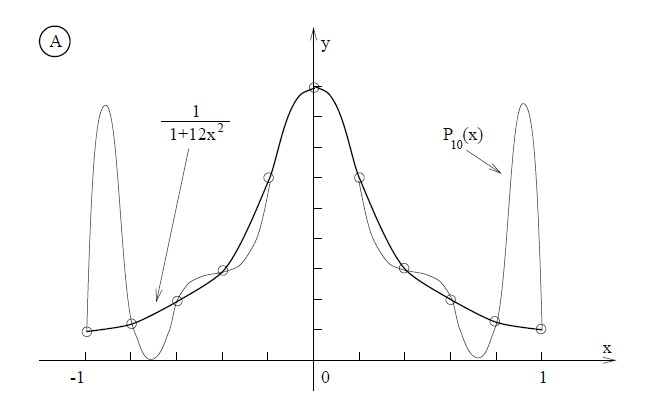
\includegraphics[height=0.8\textheight]{img/5/czebyszew.jpg}
	\end{figure}
\end{frame}
%%%%%%%%%%%%%%%%%%%
\begin{frame}{Interpolujący wielomian Czebyszewa}
	$T_n(x)$ zachowują się równomiernie w $[-1,1]$; min = -1, max = 1 - \textbf{ważna własność} \newline
    Do utworzenia wielomianu interpolacyjnego używamy liniowej kombinacji:
    $$W_n(x) = \sum_{j=0}^{N}c_jT_j(x)$$
    $\{c_j\}$ - z własności ortogonalności dla przypadku dyskretnego:
    $$x_k=\cos\Big(\frac{2k+1}{N+1}\frac{\pi}{2}\Big)\rightarrow \text{zera } T_{N+1}(x),k=0,1,..,N$$
    $$\sum_{k=0}^{N}T_i(x_k)T_j(x_k) = \left\{\begin{array}{cc}
    	0 & i \not= j \\
        N+1 & i=j=0 \\
        \frac{N+1}{2} & i=j\not=0
    \end{array}\right.$$
\end{frame}
%%%%%%%%%%%%%%%%%%%
\begin{frame}{Warunek interpolacji}
	$$f(x_k)= \sum_{j=0}^{N}c_jT_j(x_k)\Bigg\arrowvert T_i(x_k)) \Bigg\arrowvert \sum_{k=0}^{N}$$
    $$\sum_{k=0}^{N}f(x_k)T_i(x_k)=\sum_{j=0}^{N}c_j\underbrace{\sum_{k=0}^{N}T_i(x_k)T_j(x_k)}_{\text{ortogonalność}}$$
\end{frame}
%%%%%%%%%%%%%%%%%%%
\begin{frame}
	\begin{figure}
		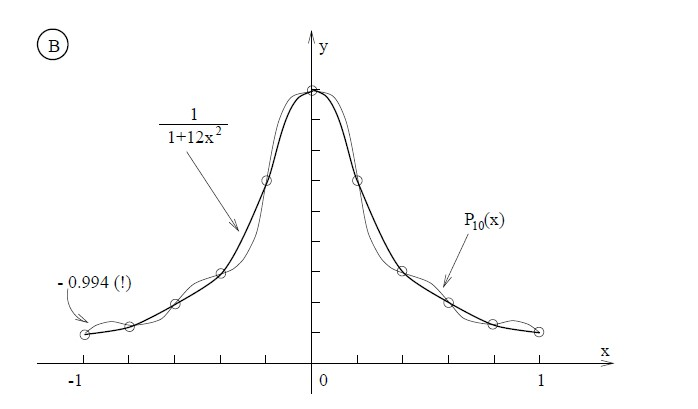
\includegraphics[height=0.8\textheight]{img/5/interpolacja.jpg}
	\end{figure}
\end{frame}
\begin{frame}{Współczynniki $c_i$}
	$$c_0 = \frac{1}{N+1}\sum_{k=0}^{N}f(x_k)T_0(x)=1$$
    $$c_i = \frac{2}{N+1}\sum_{k=0}^{N}f(x_k)T_i(x_k)$$
    Pozostaje nam wyliczenie sumy.
\end{frame}
%%%%%%%%%%%%%%%%%%%

    \section{Wzór rekurencyjny Clenshawa}
%%%%%%%%%%%%%%%%%%%
\begin{frame}{Clenshaw's recurrence formula}
	- elegancki i efektywny sposób sumowania wyrazów spełniających pewien wzór rekurencyjny:
    $$f(x) = \sum_{k=0}^{N}c_kF_k(x)$$
    przy czym $F(x)$ - spełnia wzór rekurencyjny:
    $$F_{n+1}(x) = \alpha(n,x) \cdot F_n(x) + \beta(n,x) \cdot F_{n-1}(x)$$
    $\alpha(n,x),\beta(n,x)$ - pewne funkcje\newline
    Określamy rekurencyjnie $y_k,k = N,N-1,..,1$ (downward order; k - decreasing) jako:
    $$y_{N+2}=y_{N+1} = 0, y_k(x) = \alpha(k,x) \cdot y_{k+1}+\beta(k+1,x) \cdot y_{k+2}+c_k$$
    stąd: $c_k = y_k - \alpha(k,x) \cdot y_{k+1} - \beta(k+1,x) \cdot y_{k+2}$ \newline
\end{frame} 
%%%%%%%%%%%%%%%%%%%
\begin{frame}
	Po podstawieniu:
    $$f(x) = \sum_{k=N}^{0}[y_k-\alpha(k,x)y_{k+1}-\beta(k+1,x)y_{k+2}] \cdot F_k(x) = $$
    $$\left.\begin{array}{rcccccl}
    	=[ & y_N & - & 0 & - & 0 & ] F_N(x) \\
        +[ &y_{N-1}& - & \alpha(N-1,x)\cdot y_N & - & 0 & ] F_{N-1}(x) \\
         & \ldots & & \ldots & & \ldots & \\
         +[ & y_8 & - & \alpha(8,x)y_9 & - & \beta(9,x)y_{10} & ] F_8(x) \\
		+[ & y_7 & - & \alpha(7,x)y_8 & - & \beta(8,x)y_9 & ] F_7(x) \\
        +[ & y_6 & - & \alpha(6,x)y_7 & - & \beta(7,x)y_8 & ] F_6(x) \\
        +[ & y_5 & - & \alpha(5,x)y_6 & - & \beta(6,x)y_7 & ] F_5(x) \\
         & \ldots & & \ldots & & \ldots & \\
		+[ & y_2 & - & \alpha(2,x)y_3 & - & \beta(3,x)y_4 & ] F_2(x) \\
        +[ & y_1 & - & \alpha(1,x)y_2 & - & \beta(2,x)y_3 & ] F_1(x) \\
        +[ & y_0 & - & \alpha(0,x)y_1 & - & \beta(1,x)y_2 & ] F_0(x) =
    \end{array}\right.$$
\end{frame}
%%%%%%%%%%%%%%%%%%%
\begin{frame}
	$$=\beta(1,x_0) \cdot y_2 \cdot F_0(x)+F_1(x) \cdot y_1(x) +F_0(x) \cdot c_0 $$
    wyznaczanie $f(x) = \sum_{k=0}^{N}c_kF_k(x)$ \newline
    dla $F_k(x)$: $F_{n+1}(x) = \alpha(n,x) \cdot F_n(x) + \beta(n,x) \cdot F_{n-1}(x)$ \newline
    sprowadza się do:
    \begin{enumerate}
    \item wyznaczenia $y_1$ i $y_2$ z formuły rekurencyjnej: \newline
    	$$\left\{\begin{array}{l}
    	y_{N+2} = y_{N+1} = 0 \\
        y_k(x) = \alpha(k,x) \cdot y_{k+1} + \beta(k+1,x) \cdot y_{k+2} +c_k
    	\end{array}\right.$$
     \item obliczenia sumy \newline
     $$f(x) = \beta(1,x) \cdot y_2(x) \cdot F_0(x) + y_1(x) \cdot F_1(x) + c_0 \cdot F_0(x)$$
    \end{enumerate}
\end{frame}
%%%%%%%%%%%%%%%%%%%
\begin{frame}{Istota wzoru}
	Na każdym etapie działanie wszystkich poprzednich $c_k \rightarrow$ 2 współczynniki, przez które mnoży się $F_{k+1},F_k$ ( $\rightarrow$ na końcu: $F_1$ i $F_0$).\newline
    Jeżeli:
    $$\left.\begin{array}{cl}
    	F_k(x) & \text{małe dla dużych k} \\
        c_k & \text{małe dla dużych k}
    \end{array}\right\} \Rightarrow\left.\begin{array}{c}
    	 \text{suma określona będzie} \\
         \text{przez małe} F_k(x)
    \end{array}\right.$$
    pamiętane współczynniki = rezultat ``delicate cancelation'' \newline
    wykrywanie: $\beta(1,x) \cdot y_2 \cdot F_0,y_1 \cdot F_1$ - przeciwnych znaków i prawie równe
\end{frame}
%%%%%%%%%%%%%%%%%%%
\begin{frame}
	Wtedy stosować \textbf{Clenshaw's recurrence in upward direction:}
    $$y_{-2} = y_{-1} = 0$$
    $$y_k = \frac{1}{\beta(k+1,x)}[y_{k-2}-\alpha(k,x)y_{k-1} - c_k], k=0,1..,N-1$$
    $$f(x) = c_NF_N(x) - \beta(B,x)F_{N-1}(x)y_{N-1} - F_N(x)y_{N-2}$$
    \begin{flushright}
    	\textit{Zadanie: } \quad Sprawdzić wzory Clenshaw'a dla $T_n(x)$ i $P_n(x)$.
    \end{flushright}
\end{frame}
%%%%%%%%%%%%%%%%%%%


\end{document}
